This chapter presents the implementation details of the SmartGrid AI Audit Framework. It covers the system environment and technology stack, the data representation scheme for the 100-agent smart grid, the algorithmic flow of the live detection pipeline, the mathematical formulations behind each computational stage, the integration workflow connecting all subsystems, and the feature-wise functional mapping used throughout the framework. The implementation turns the conceptual framework proposed by Priyadarsini~\cite{priyadarsini2025} into a fully working platform.

%---------------------------------------------------------------------
\section{System Environment and Technology Stack}
\label{sec:tech_stack}
%---------------------------------------------------------------------

The framework is implemented using a modular stack comprising a Python-based backend, a JavaScript-based frontend, a SCADA supervisory layer, a data acquisition bridge, and local storage. All components are executed on a standard workstation without the requirement of a dedicated GPU, making it easy to reproduce and run.

\par \vspace{0.35cm}
\noindent
\textbf{Backend: FastAPI (Python):} The core backend is built using FastAPI, a high-performance Python web framework based on ASGI. It exposes REST endpoints for SCADA data ingestion, anomaly scoring, multi-layer detection, audit scheduling, and explainability (XAI) output. FastAPI was selected for its native support of asynchronous request handling, automatic OpenAPI documentation, and compatibility with the scientific Python ecosystem.

\par \vspace{0.35cm}
\noindent
\textbf{Frontend: Next.js Dashboard:} The operator-facing interface is implemented as a Next.js application (React-based framework). The dashboard is organised into two distinct workspaces:
\begin{itemize}
    \item \textit{Experiment Running}, used for simulation, benchmarking, and comparative evaluation of detection methods.
    \item \textit{Rapid SCADA Live}, used for real-time monitoring of the 100-agent grid, displaying live telemetry, anomaly flags, audit decisions, and explainability outputs.
\end{itemize}

\par \vspace{0.35cm}
\noindent
\textbf{SCADA Layer: Rapid SCADA:} Rapid SCADA Webstation serves as the supervisory telemetry layer~\cite{martinelli2022method}. The Rapid SCADA Web API, accessible at \texttt{127.0.0.1:10109}, provides authenticated access to channel data. A total of 670 calculated channels are configured across two configuration files, \texttt{Cnl.xml} for physical channels and \mbox{\texttt{Cnl\_Cyber\_Addon.xml}} for cyber channels, to represent the telemetry of the 100-agent grid. Generators use channels 101--160 (physical) and 501--580 (cyber), substations use 201--290 and 601--690, PMUs use 301--375 and 701--800, and breakers use 401--475 and 801--900. Calculated channels were used rather than input channels because input channels in Rapid SCADA require physical device connections, whereas calculated channels allow programmatic generation of telemetry values within the SCADA environment.

\par \vspace{0.35cm}
\noindent
\textbf{Data Acquisition Bridge: PowerShell Script:} A PowerShell script serves as the bridge between Rapid SCADA and the FastAPI backend. The bridge script (\mbox{\texttt{pull\_rapidscada\_to\_api.ps1}}) authenticates with the Rapid SCADA Web API, retrieves telemetry values in batch, and transmits them to the backend ingestion endpoint~\cite{martinelli2022method}. This approach decouples the SCADA layer from the backend, allowing independent operation and testing of each component.

\par \vspace{0.35cm}
\noindent
\textbf{Machine Learning: PyTorch:} All LSTM-based temporal detection models are implemented using PyTorch. The dual-branch LSTM architecture (grid branch and network branch) is trained and executed entirely within the Python backend. PyTorch was chosen for its dynamic computation graph, ease of debugging, and compatibility with the rest of the Python stack.

\par \vspace{0.35cm}
\noindent
\textbf{Database: SQLite:} SQLite is used for persistent storage of the audit chain and telemetry records. The audit chain database (\texttt{audit\_chain.db}) stores all audit decisions, anomaly flags, risk scores, and scheduling outcomes. SQLite was selected for its zero-configuration deployment, single-file storage, and suitability for single-machine operation without a dedicated database server.

\par \vspace{0.35cm}
\noindent
\textbf{Execution Environment:} The entire framework operates on a standard workstation. No GPU acceleration is required for inference or training at the current 100-agent scale. This design choice ensures that the system can be reproduced and evaluated without specialised hardware.

\begin{figure}[H]
\centering
\fbox{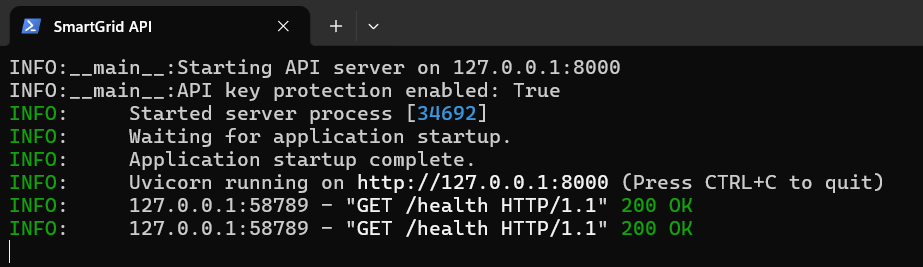
\includegraphics[width=0.95\textwidth]{SmartGridAPI.png}}
\caption{FastAPI backend running with all REST endpoints for SCADA ingestion, anomaly detection, audit scheduling, and explainability.}
\label{fig:smartgrid_api}
\end{figure}

\begin{figure}[H]
\centering
\fbox{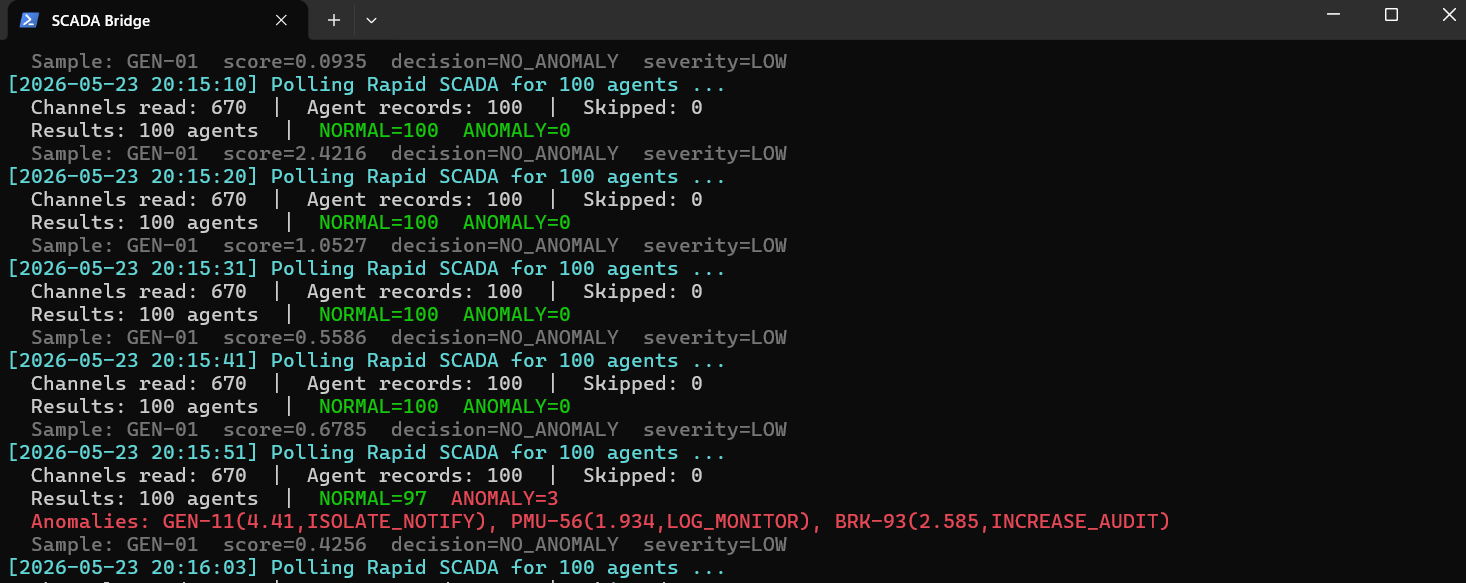
\includegraphics[width=0.95\textwidth]{SCADABridge_Terminal.png}}
\caption{PowerShell bridge terminal showing live telemetry retrieval from Rapid SCADA and batch transmission to the FastAPI backend.}
\label{fig:scada_bridge_terminal}
\end{figure}


%---------------------------------------------------------------------
\section{Smart Grid Data Representation}
\label{sec:data_representation}
%---------------------------------------------------------------------

The smart grid is modelled as a multi-agent system~\cite{farid2014multi} comprising 100 agents distributed across four functional classes. Each agent is assigned a unique identifier and a set of physical and cyber features that collectively characterise its operational state. All telemetry data used in both the experiment and SCADA live workspaces is synthetically generated: the experiment workspace uses the \texttt{GridEnvConfig}-based simulation engine (\texttt{grid\_env.py}), while the SCADA live workspace uses calculated channels within Rapid SCADA that produce programmatically generated values. No external or third-party datasets are used as the live or simulation telemetry source. However, two public benchmark datasets, the UCI Electrical Grid Stability Dataset and the UNSW-NB15 Network Intrusion Dataset, are used exclusively for LSTM model pre-training prior to fine-tuning on the synthetic grid data. This distinction is important: the datasets train the model weights, not the runtime telemetry pipeline (see Section~\ref{sec:lstm_arch_training}).

\par \vspace{0.35cm}
\noindent
\textbf{Agent Classes and Identifiers:} The 100 agents are organised into four classes as follows:
\begin{itemize}
    \item \textbf{Generators (GEN):} GEN-01 to GEN-20 (20 agents), represent power generation units.
    \item \textbf{Substations (SUB):} SUB-21 to SUB-50 (30 agents), represent power transformation and distribution nodes.
    \item \textbf{Phasor Measurement Units (PMU):} PMU-51 to PMU-75 (25 agents), represent high-frequency synchronised measurement devices.
    \item \textbf{Breakers (BRK):} BRK-76 to BRK-100 (25 agents), represent circuit protection and switching devices.
\end{itemize}

\par \vspace{0.35cm}
\noindent
\textbf{Physical Features:} Each agent reports a set of physical measurements that reflect the electrical state of the corresponding grid component. The physical feature vector $\mathbf{x} \in \mathbb{R}^{n_x}$ includes:
\begin{itemize}
    \item \textit{Voltage} (in volts), bus voltage magnitude (nominal 230\,V for generators).
    \item \textit{Current} (in amperes), line current magnitude (nominal 100\,A for generators).
    \item \textit{Frequency} (in hertz), system frequency at the measurement point (nominal 50\,Hz).
    \item \textit{Power} (in kilowatts), active power flow (derived from voltage $\times$ current $\times$ power factor).
    \item \textit{Response Time} (in milliseconds), measurement response latency of the physical sensor.
\end{itemize}

\par \vspace{0.35cm}
\noindent
\textbf{Cyber Features:} Each agent additionally reports a set of cyber (network) measurements that characterise the communication health of its telemetry channel. The cyber feature vector $\mathbf{y} \in \mathbb{R}^{n_y}$ includes:
\begin{itemize}
    \item \textit{Latency} (in milliseconds), round-trip communication delay.
    \item \textit{Packet Loss} (as a ratio), fraction of telemetry packets lost in transit.
    \item \textit{Communication Frequency} (in hertz), rate of telemetry reporting.
    \item \textit{Integrity} (as a score), computed integrity metric for the communication channel.
\end{itemize}

\par \vspace{0.35cm}
\noindent
\textbf{Rapid SCADA Channel Model:} The 100-agent grid is represented within Rapid SCADA using a total of 670 calculated channels distributed across physical and cyber configuration files. The channel allocation varies by asset class: generators receive 7 channels each (3 physical + 4 cyber), substations receive 6 channels each (3 physical + 3 cyber, with no dedicated cyber latency channel), PMUs receive 7 channels each (3 physical + 4 cyber), and breakers receive 7 channels each (3 physical + 4 cyber). As noted in Section~\ref{sec:tech_stack}, calculated channels were used in place of input channels because input channels in Rapid SCADA require connections to physical field devices, which are not present in the current deployment. Calculated channels allow the SCADA environment to generate representative telemetry values programmatically, which allows full pipeline validation without hardware dependencies.

\par \vspace{0.35cm}

\begin{figure}[H]
\centering
\fbox{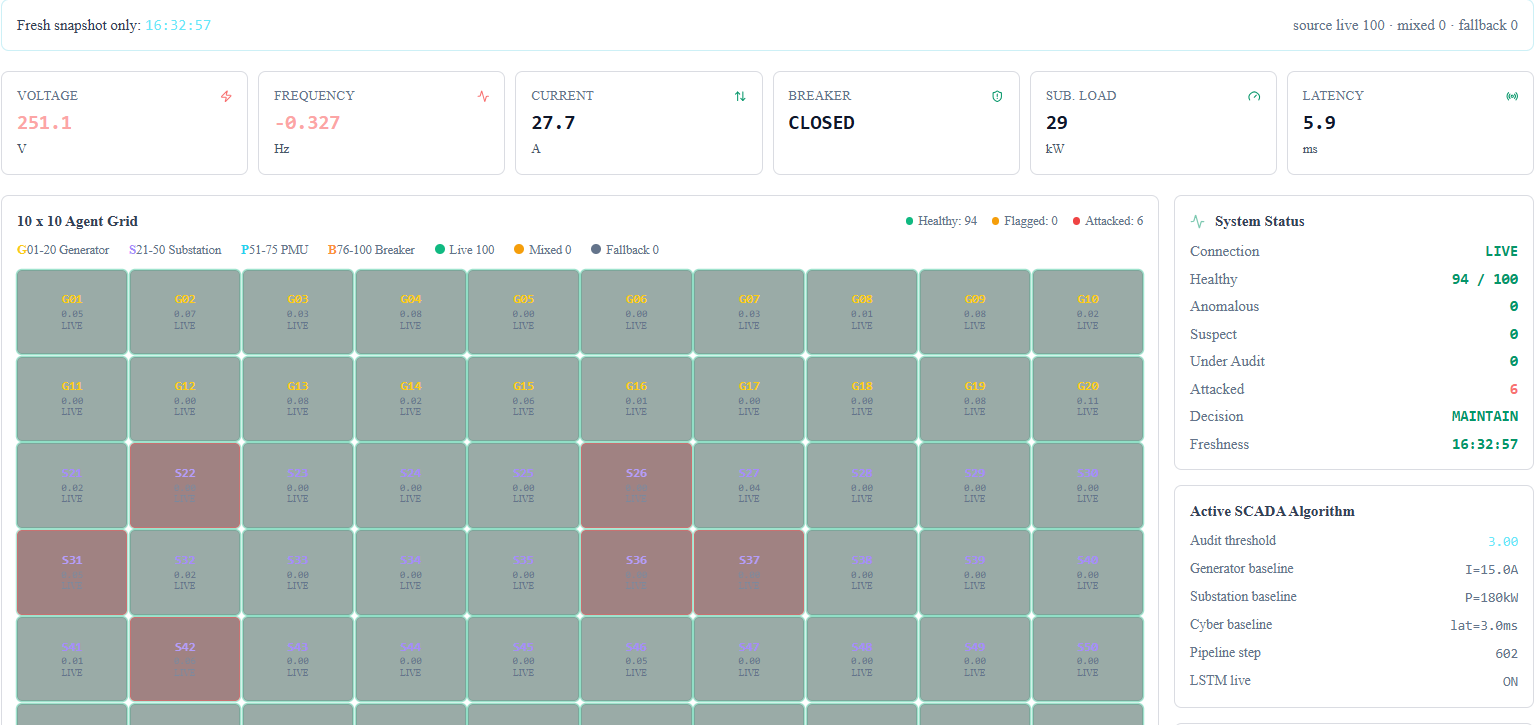
\includegraphics[width=0.95\textwidth]{FigGrid_With_The_Agents.png}}
\caption{Rapid SCADA live grid view showing the 100-agent smart grid with generators, substations, PMUs, and breakers.}
\label{fig:grid_agents}
\end{figure}

\begin{figure}[H]
\centering
\fbox{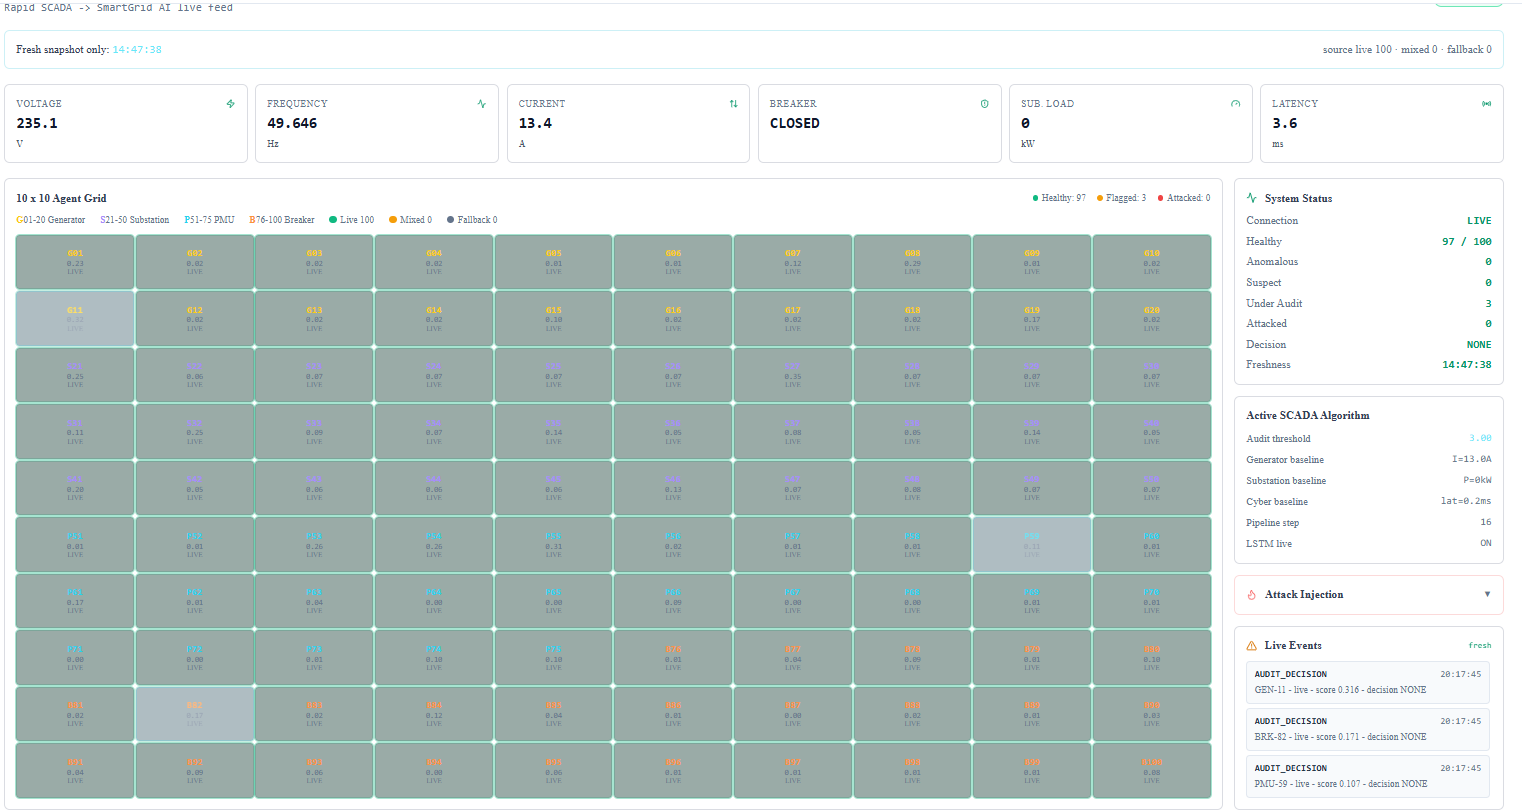
\includegraphics[width=0.95\textwidth]{FigScadaGrid_Normal.png}}
\caption{SCADA grid view during normal operation showing all agents in healthy state with no anomaly flags.}
\label{fig:scada_grid_normal}
\end{figure}

\begin{figure}[H]
\centering
\fbox{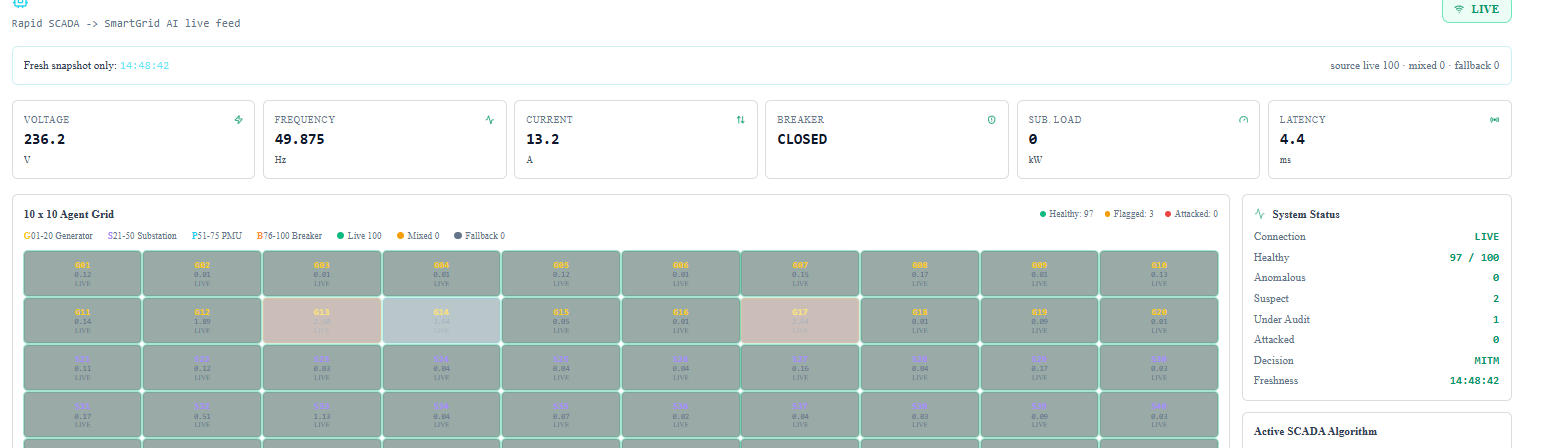
\includegraphics[width=0.95\textwidth]{FigScadaGrid_Attack.png}}
\caption{SCADA grid view during an active attack scenario showing affected agents flagged with anomaly indicators.}
\label{fig:scada_grid_attack}
\end{figure}


%---------------------------------------------------------------------
\section{Algorithmic Flow and Execution Process}
\label{sec:algo_flow}
%---------------------------------------------------------------------

The live detection pipeline follows a nine-step sequential process. Each step transforms or enriches the data, progressing from raw telemetry acquisition to final operator-facing outputs. The steps are described below.

\par \vspace{0.35cm}
\noindent
\textbf{Step 1: Data Acquisition:} Telemetry data is acquired from one of two sources depending on the active workspace. In the \textit{Experiment Running} workspace, data is generated or loaded from simulation datasets. In the \textit{Rapid SCADA Live} workspace, the PowerShell bridge (\mbox{\texttt{pull\_rapidscada\_to\_api.ps1}}) retrieves telemetry from the Rapid SCADA Web API at \texttt{127.0.0.1:10109} and transmits it to the FastAPI backend in batch form. This step produces the raw physical feature vector $\mathbf{x}$ and cyber feature vector $\mathbf{y}$ for each agent.

\par \vspace{0.35cm}
\noindent
\textbf{Step 2: Observation:} Each agent executes an observation step via the method \texttt{agent.observe($\mathbf{x}_{\text{phys}}$, $\mathbf{y}_{\text{cyber}}$)}. This method registers the incoming physical and cyber feature vectors into the agent's internal state, making them available for subsequent scoring and detection operations. The observation step also updates the agent's telemetry history buffer, which is used by the LSTM temporal model.

\par \vspace{0.35cm}
\noindent
\textbf{Step 3: LSTM Inference:} A dual-branch LSTM model processes the agent's recent telemetry history. The grid branch analyses physical features to produce a grid anomaly probability, while the network branch analyses cyber features to produce a network intrusion probability. The two branch outputs are combined using the function \mbox{\texttt{fuse\_branch\_probabilities()}} with fusion weights $w_{\text{grid}} = 0.58$ and $w_{\text{network}} = 0.42$, yielding a unified anomaly probability $p_{\text{anomaly}} \in [0,1]$. This picks up patterns that instantaneous deviation scoring alone would miss.

\par \vspace{0.35cm}
\noindent
\textbf{Step 4: Scoring:} The function \texttt{compute\_score\_and\_flag()} calculates the agent's composite risk score and binary anomaly flag. This step proceeds as follows:
\begin{enumerate}
    \item \textit{EWMA Drift Compensation:} Before deviation scoring, a slow drift correction is applied to prevent the scorer from raising false alarms during gradual but legitimate load shifts. An exponentially weighted moving average (EWMA) with smoothing factor $\alpha_{\text{ewma}} = 0.30$ tracks the rolling mean of each feature over a window of 24 timesteps. When the rolling mean drifts from the static baseline by more than a marginal amount, 30\% of that difference is subtracted from the observed value prior to computing the normalised deviation. This keeps the effective deviation centred on the true short-term operating point rather than the fixed installation-time baseline.
    \item \textit{Deviation Scoring:} The physical deviation $d_x$ and cyber deviation $d_y$ are computed as the root-mean-square of the EWMA-compensated normalised feature deviations from the agent's baseline (see Equations~\ref{eq:dx} and~\ref{eq:dy}). The composite score is $S_i(t) = w_i \cdot (d_x + d_y)$, where $w_i$ is the agent's criticality weight (Equation~\ref{eq:si}).
    \item \textit{Weighted Ensemble:} The hybrid confidence score combines deviation-based and LSTM-based evidence:
    \begin{equation}
    \text{hybrid\_conf} = 0.48 \cdot \text{dev\_conf} + 0.52 \cdot \text{prob\_support} + \text{suspicion\_credit}
    \label{eq:hybrid_inline}
    \end{equation}
    where the weights 0.48 and 0.52 reflect the validated configuration giving slightly greater emphasis to the temporal LSTM detector.
    \item \textit{Binary Flag:} The anomaly flag $a_i(t)$ is set to 1 if the combined conditions on deviation magnitude and hybrid confidence exceed the agent's calibrated thresholds, and 0 otherwise.
\end{enumerate}

\par \vspace{0.35cm}
\noindent
\textbf{Detection Sensitivity Profiles.} The system supports three named runtime profiles that adjust the primary detection thresholds without retraining any model component. Each profile trades sensitivity against false positive tolerance according to operational requirements:

\begin{itemize}
    \item \textit{ROBUST}, $k_\sigma = 3.5$, deviation score threshold $= 3.60$, LSTM probability threshold $= 0.80$. This profile is the most sensitive and is suited for high-security environments where the cost of a missed attack outweighs the nuisance of occasional false alarms.
    \item \textit{BALANCED}, $k_\sigma = 4.0$, deviation score threshold $= 3.85$, LSTM probability threshold $= 0.85$. This is the default operational profile and provides the best overall F1 score across the evaluated scenarios.
    \item \textit{COST}, $k_\sigma = 5.0$, deviation score threshold $= 4.10$, LSTM probability threshold $= 0.90$. This profile minimises audit expenditure by raising the evidence bar for flagging an agent, and is appropriate when audit resources are constrained and the expected attack rate is low.
\end{itemize}

The $k_\sigma$ parameter scales the adaptive threshold used in the sigma-window computation, where the threshold for each feature is $\tau = k_\sigma \cdot \hat{\sigma}$ and $\hat{\sigma}$ is the empirical standard deviation over the most recent 24-timestep window.

\par \vspace{0.35cm}
\noindent
\textbf{Step 5: Multi-Layer Detection:} A three-layer detection architecture provides defence in depth:
\begin{enumerate}
    \item \textbf{Layer 1: Calibrated LSTM Threshold:} The LSTM anomaly probability is compared against a calibrated per-agent threshold. Agents whose $p_{\text{anomaly}}$ exceeds the threshold are flagged at this layer.
    \item \textbf{Layer 2: Temporal Accumulator:} A sliding-window accumulator tracks the frequency of anomaly flags over recent time steps. Agents exhibiting sustained anomalous behaviour (i.e., repeated flags within the accumulation window) are escalated, even if individual flags are marginally above the threshold.
    \item \textbf{Layer 3: Specialised Attack Detectors:} Four attack-specific detectors operate in parallel:
    \begin{itemize}
        \item \textit{CUSUM Detector}, for false data injection (FDI) attacks~\cite{liu2009false}, based on cumulative sum change-point detection on physical feature residuals, with a shape gate that requires the latest residual to match the FDI pattern before the detector fires.
        \item \textit{DoS Detector}, for denial-of-service attacks, based on rule-based evaluation of communication frequency drops and packet loss spikes.
        \item \textit{MITM Detector}, for man-in-the-middle attacks, based on integrity score degradation and latency anomalies.
        \item \textit{Fault Signature Detector}, for physical faults (voltage sag, overcurrent, and frequency deviation), based on template matching when one physical feature stands out while the cyber channels stay quiet. This detector takes precedence over the CUSUM detector when both fire, so a fault is not mislabelled as an FDI attack.
    \end{itemize}
    A cross-layer corroboration check then drops a deviation-only flag when neither the LSTM nor any of the four detectors agrees with it, which lowers the false alarm rate.
\end{enumerate}

\par \vspace{0.35cm}
\noindent
\textbf{Step 6: Behaviour Update:} After detection, each agent refines its internal baseline and detection thresholds. Baseline values are updated using an exponential moving average with smoothing factor $\alpha = 0.1$, applied \textit{only when the anomaly flag is zero} (i.e., during normal conditions). During detected anomalies, baselines are frozen to prevent contamination from attack-corrupted observations. This guard ensures that sustained attacks cannot gradually shift the baseline toward malicious values. Detection thresholds are adjusted based on the observed false positive rate and detection sensitivity, so that the system stays calibrated over time.

\par \vspace{0.35cm}
\noindent
\textbf{Step 7: Audit Scheduling:} The hybrid audit scheduler determines the audit frequency for each agent using two complementary mechanisms:
\begin{itemize}
    \item \textit{Reinforcement Learning (Q-Learning):} A Q-table maps agent risk states to audit frequency actions. The Q-values are updated after each audit decision based on the observed reward, which balances detection effectiveness against audit cost.
    \item \textit{Gradient-Based Cost Optimisation:} The audit frequency is further refined by minimising a cost function that balances audit cost against expected risk exposure. The gradient of this cost function with respect to audit frequency is computed analytically and used to update the frequency through gradient descent (see Section~\ref{sec:gradient_audit}).
\end{itemize}
The function \texttt{hybrid\_audit\_schedule()} combines the outputs of both mechanisms to produce the final audit frequency for each agent.

\par \vspace{0.35cm}
\noindent
\textbf{Step 8: Response and Action Escalation:} Based on the detection results and audit decisions, the system selects one of five escalation levels for each agent:
\begin{itemize}
    \item \texttt{NO\_ANOMALY}, normal operation; no action required.
    \item \texttt{LOG\_MONITOR}, marginal deviation; event is logged and passive monitoring is enhanced.
    \item \texttt{INCREASE\_AUDIT}, elevated monitoring; audit frequency is increased.
    \item \texttt{ISOLATE\_NOTIFY}, the agent is flagged for isolation and the operator is notified.
    \item \texttt{EMERGENCY\_SHUTDOWN}, critical threat; immediate shutdown action is recommended.
\end{itemize}

\par \vspace{0.35cm}
\noindent
\textbf{Step 9: XAI Output:} The explainability module invokes \texttt{explain\_deviation()} independently for physical and cyber feature domains. For each domain, the module computes per-feature contribution scores (see Section~\ref{sec:xai_formulas}) and identifies the top contributing features driving the anomaly flag. The output is a ranked list of features with their relative contributions, presented to the operator through the dashboard.

\begin{figure}[H]
\centering
\fbox{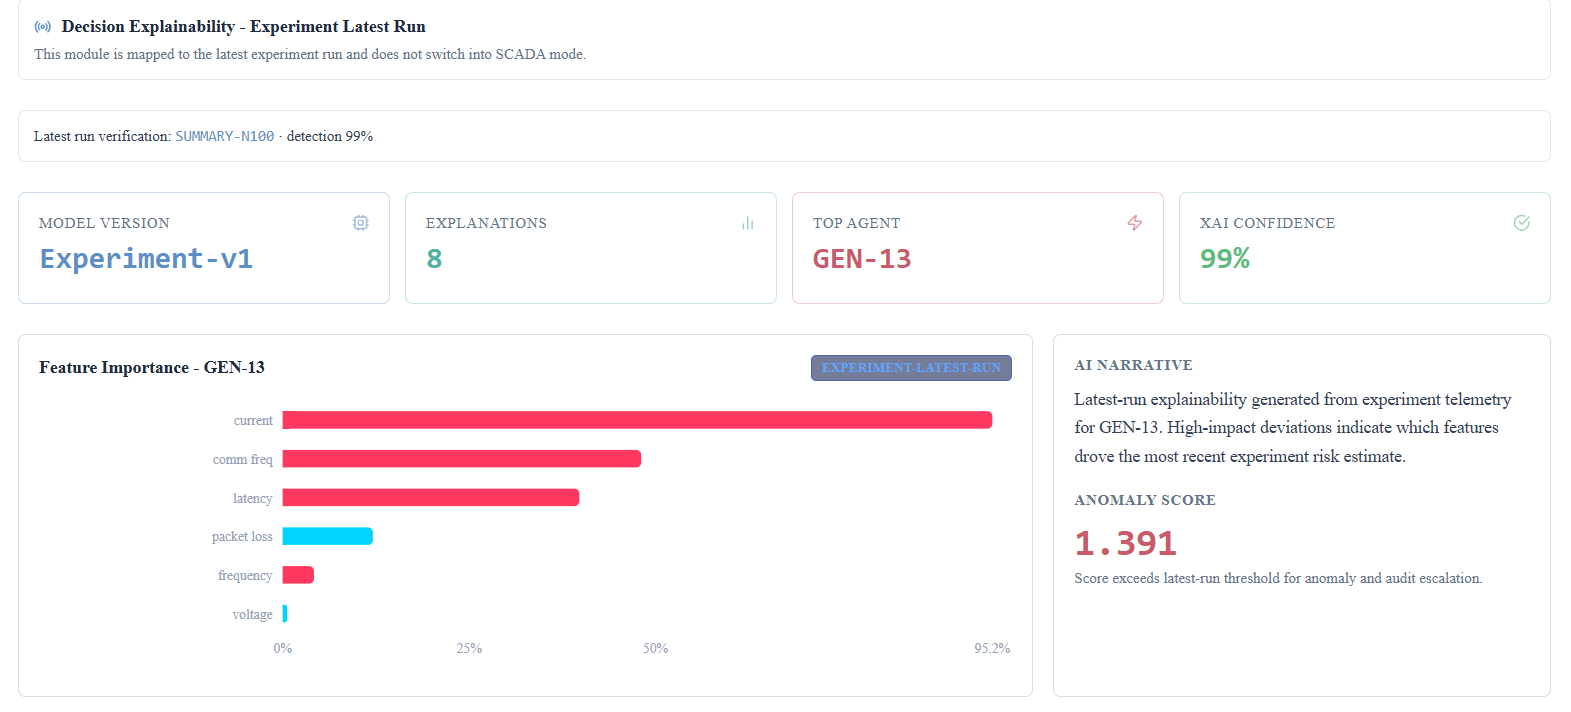
\includegraphics[width=0.95\textwidth]{FigExperiment_Decision_Explainability.png}}
\caption{Explainability (XAI) view showing per-feature deviation contributions for a selected agent, with physical and cyber domains displayed independently.}
\label{fig:xai_view}
\end{figure}


%---------------------------------------------------------------------
\section{Mathematical Formulations}
\label{sec:math_formulations}
%---------------------------------------------------------------------

This section presents the mathematical formulations underlying the key computational stages of the framework. All equations use consistent notation: $\mathbf{x}$ denotes physical features, $\mathbf{y}$ denotes cyber features, $\mathbf{b}$ denotes baseline values, and $\boldsymbol{\theta}$ denotes threshold values.

%.....................................................................
\subsection{Deviation Scoring Formulas}
\label{sec:deviation_formulas}
%.....................................................................

The deviation scoring module, adapted from the formulation in~\cite{priyadarsini2025}, quantifies how far an agent's current observations deviate from its learned baseline. The normalised z-score for a single feature observation is defined as:
\begin{equation}
z = \frac{\text{obs} - \text{base}}{\theta}
\label{eq:z}
\end{equation}
where $\text{obs}$ is the observed value, $\text{base}$ is the baseline value, and $\theta$ is the corresponding threshold.

\par \vspace{0.25cm}
\noindent
The physical deviation $d_x$ aggregates the normalised deviations across all physical features:
\begin{equation}
d_x = \sqrt{ \frac{1}{n_x} \sum_{j=1}^{n_x} \left( \frac{x_j - b_{x,j}}{\theta_{x,j}} \right)^2 }
\label{eq:dx}
\end{equation}
where $n_x$ is the number of physical features, $x_j$ is the observed value of the $j$-th physical feature, $b_{x,j}$ is its baseline, and $\theta_{x,j}$ is its threshold.

\par \vspace{0.25cm}
\noindent
Similarly, the cyber deviation $d_y$ is computed over all cyber features:
\begin{equation}
d_y = \sqrt{ \frac{1}{n_y} \sum_{j=1}^{n_y} \left( \frac{y_j - b_{y,j}}{\theta_{y,j}} \right)^2 }
\label{eq:dy}
\end{equation}
where $n_y$ is the number of cyber features, $y_j$ is the observed value of the $j$-th cyber feature, $b_{y,j}$ is its baseline, and $\theta_{y,j}$ is its threshold.

\par \vspace{0.25cm}
\noindent
The composite deviation score for agent $i$ at time $t$ is:
\begin{equation}
S_i(t) = w_i \cdot (d_x + d_y)
\label{eq:si}
\end{equation}
where $w_i$ is the criticality weight assigned to agent $i$ based on its class (generator, substation, PMU, or breaker).

%.....................................................................
\subsection{LSTM Ensemble and Hybrid Confidence}
\label{sec:hybrid_confidence}
%.....................................................................

The hybrid confidence score combines evidence from the deviation-based detector and the LSTM-based temporal detector using a weighted ensemble:
\begin{equation}
\text{hybrid\_conf} = w_{\text{dev}} \cdot \text{dev\_conf} + w_{\text{prob}} \cdot \text{prob\_support} + \text{suspicion\_credit}
\label{eq:hybrid}
\end{equation}
where $w_{\text{dev}} = 0.48$ is the deviation confidence weight, $w_{\text{prob}} = 0.52$ is the LSTM probability weight, $\text{dev\_conf}$ is the confidence derived from deviation magnitude, $\text{prob\_support}$ is the LSTM anomaly probability, and $\text{suspicion\_credit}$ is an additional term accumulated from the temporal accumulator when sustained anomalous behaviour is observed.

\par \vspace{0.25cm}
\noindent
The binary anomaly flag for agent $i$ at time $t$ is determined as:
\begin{equation}
a_i(t) =
\begin{cases}
1, & \text{if the combined conditions on deviation magnitude and} \\
   & \text{hybrid confidence exceed the calibrated thresholds} \\
0, & \text{otherwise}
\end{cases}
\label{eq:ai}
\end{equation}

%.....................................................................
\subsection{LSTM Architecture and Training Methodology}
\label{sec:lstm_arch_training}
%.....................................................................

\textbf{Model Architecture.} Each branch of the dual-branch LSTM is a two-layer LSTM with 64 hidden units per layer and a dropout of 0.20 between layers. A single fully-connected output layer maps the last hidden state to one logit, and a sigmoid activation converts that logit to a probability in $[0,1]$. Temporal input sequences are formed by a sliding window of 24 consecutive timesteps, giving each training sample the shape $(24,\, n_{\text{feat}})$. The window size of 24 captures one short-term operational cycle at the standard SCADA polling interval and was validated to provide stable gradient flow without overfitting. The data is split 80\% for training and 20\% for validation. Training uses the Adam optimiser at a learning rate of $10^{-3}$, a batch size of 64, and runs for up to 20 epochs.

\par \vspace{0.35cm}
\noindent
\textbf{Pre-Training Datasets.} The dual-branch LSTM is pre-trained on two publicly available benchmark datasets before fine-tuning on the synthetic grid simulation data. The pre-training step gives each branch a meaningful starting point that reflects real-world physical and network dynamics, reducing the amount of synthetic data needed to reach convergence.

\par \vspace{0.25cm}
\noindent
\textit{UCI Electrical Grid Stability Dataset (Dataset \#471).} The physical grid branch is pre-trained on the UCI Electrical Grid Stability Dataset, which contains 10{,}000 samples with 12 numerical features: four producer reaction times (\texttt{tau1}--\texttt{tau4}), four power balance coefficients (\texttt{p1}--\texttt{p4}), and four price elasticity coefficients (\texttt{g1}--\texttt{g4}). The binary stability label (stable / unstable) serves as the pre-training target. The continuous regression column \texttt{stab} is excluded, and any missing values are filled using per-feature median imputation. The dataset models a four-node power network under varying supply-demand conditions, which means the physical branch learns the characteristic dynamics of voltage and frequency imbalance before it ever sees a smart grid observation. Table~\ref{tab:uci_feature_map} shows how the UCI feature groups map onto the physical features of the grid simulation.

\begin{table}[H]
\centering
\caption{UCI Electrical Grid Stability Dataset: feature-to-simulation mapping.}
\label{tab:uci_feature_map}
\begin{tabular}{|l|l|l|}
\hline
\textbf{UCI Feature Group} & \textbf{UCI Columns} & \textbf{Simulation Mapping} \\
\hline
Producer reaction times & \texttt{tau1}--\texttt{tau4} & Physical response latency \\
Power balance & \texttt{p1}--\texttt{p4} & Voltage and power deviations \\
Price elasticity & \texttt{g1}--\texttt{g4} & Frequency and current load sensitivity \\
\hline
\end{tabular}
\end{table}

\par \vspace{0.25cm}
\noindent
\textit{UNSW-NB15 Network Intrusion Dataset.} The network/cyber branch is pre-trained on the UNSW-NB15 dataset. Rather than feeding in the raw 47-feature vector, four composite engineered features are derived that correspond one-to-one with the four cyber features used in the simulation:

\begin{enumerate}
    \item $\text{latency\_like} = \ln\!\left(1 + \texttt{dur} + \texttt{tcprtt} + \texttt{synack} + \texttt{ackdat} + \texttt{sinpkt} + \texttt{dinpkt} + \texttt{sjit} + \texttt{djit}\right)$
    \item $\text{loss\_like} = \ln\!\left(1 + \texttt{sloss} + \texttt{dloss} + \text{pkt\_correction}\right)$
    \item $\text{integrity\_like} = \ln\!\left(1 + |\texttt{sttl} - \texttt{dttl}| + \texttt{ct\_state\_ttl} + \tfrac{|\texttt{sbytes} - \texttt{dbytes}|}{\max(\texttt{sbytes}+\texttt{dbytes},\, 1)}\right)$
    \item $\text{freq\_like} = \ln\!\left(1 + \texttt{rate} + \texttt{sload} + \texttt{dload} + \texttt{spkts} + \texttt{dpkts}\right)$
\end{enumerate}

The $\ln(1+x)$ transform compresses the heavy-tailed distributions typical of network flow data. Each composite is then z-score normalised across the dataset. The mapping is deliberate: \textit{latency\_like} aggregates timing and inter-packet gap signals, mapping to the \textit{latency} cyber feature; \textit{loss\_like} captures retransmission and packet drop patterns, mapping to \textit{packet loss}; \textit{integrity\_like} reflects header discrepancies and data consistency deviations, mapping to \textit{integrity}; and \textit{freq\_like} captures throughput and rate, mapping to \textit{communication frequency}. The binary label (\texttt{label} $> 0$ = attack) trains the cyber branch to distinguish normal network flows from intrusion patterns. Table~\ref{tab:unsw_feature_map} summarises the correspondence.

\begin{table}[H]
\centering
\caption{UNSW-NB15 engineered features and their cyber feature mappings.}
\label{tab:unsw_feature_map}
\begin{tabular}{|l|l|l|}
\hline
\textbf{Engineered Feature} & \textbf{Source Fields (UNSW-NB15)} & \textbf{Simulation Cyber Feature} \\
\hline
\textit{latency\_like} & \texttt{dur, tcprtt, synack, ackdat, sinpkt, dinpkt, sjit, djit} & Latency \\
\textit{loss\_like} & \texttt{sloss, dloss}, packet mismatch & Packet Loss \\
\textit{integrity\_like} & \texttt{sttl, dttl, ct\_state\_ttl, sbytes, dbytes} & Integrity \\
\textit{freq\_like} & \texttt{rate, sload, dload, spkts, dpkts} & Communication Frequency \\
\hline
\end{tabular}
\end{table}

\par \vspace{0.35cm}
\noindent
\textbf{Handling Class Imbalance.} Attack events are rare relative to normal operating time, so training data is skewed heavily toward the negative class. Two techniques are combined to address this. \textit{Focal Loss} replaces standard binary cross-entropy as the training objective:
\begin{equation}
\mathcal{L}_{\text{focal}} = -\alpha \left(1 - p_t\right)^{\gamma} \log(p_t)
\label{eq:focal}
\end{equation}
where $p_t$ is the model's estimated probability for the ground-truth class, $\alpha = 0.65$ is the class weight assigned to the positive (attack) class, and $\gamma = 2.0$ is the focusing exponent. The factor $(1 - p_t)^\gamma$ reduces the loss contribution from easy well-classified samples and concentrates the gradient on harder minority-class examples. Alongside Focal Loss, a \textit{WeightedRandomSampler} oversamples the minority class during batch construction using a positive-class scale factor of 1.40 and an oversampling scale of 1.35, so attack samples appear more frequently within each mini-batch.

\par \vspace{0.35cm}
\noindent
\textbf{Temperature Calibration.} Raw LSTM output probabilities are often poorly calibrated: a predicted value of 0.80 does not necessarily correspond to an 80\% empirical likelihood of attack. After training, a post-hoc temperature calibration step is performed on the held-out validation set. A temperature parameter $T$ is selected by grid search over $T \in [0.80,\, 2.20]$ in increments of 0.05, simultaneously with a decision threshold search over $[0.40,\, 0.65]$. The pair $(T^*, \text{threshold}^*)$ that jointly maximises the validation F1 score and minimises the Brier score (a calibration loss) is saved in the model checkpoint. During inference, the raw logit $z$ is divided by $T^*$ before the sigmoid activation, producing a calibrated probability that is well-suited for its 0.52-weighted contribution to the hybrid confidence ensemble in Equation~\ref{eq:hybrid}.

%.....................................................................
\subsection{Explainability Formulas}
\label{sec:xai_formulas}
%.....................................................................

The explainability module computes per-feature contribution scores to identify which features are most responsible for a given anomaly flag. For each feature $j$ in the physical domain, the squared normalised contribution is:
\begin{equation}
c_j = \left( \frac{x_j - b_j}{\theta_j} \right)^2
\label{eq:cj}
\end{equation}

\par \vspace{0.25cm}
\noindent
The relative contribution of feature $j$ is then:
\begin{equation}
\text{relative}_j = \frac{c_j}{\displaystyle\sum_{k=1}^{n} c_k}
\label{eq:rel}
\end{equation}
where $n$ is the total number of features in the domain. An analogous computation is performed for cyber features using $\mathbf{y}$, $\mathbf{b}_y$, and $\boldsymbol{\theta}_y$. The features with the highest relative contributions are reported in ranked order as the explanation for the anomaly flag.

%.....................................................................
\subsection{Gradient Audit Optimisation}
\label{sec:gradient_audit}
%.....................................................................

The gradient-based audit optimisation module determines the optimal audit frequency for each agent by minimising a cost function that balances audit expenditure against risk exposure. The cost function for agent $i$ is:
\begin{equation}
C_i = C_a \cdot f_i + C_f \cdot \frac{R_i}{f_i}
\label{eq:ci}
\end{equation}
where $C_a$ is the per-audit cost, $f_i$ is the audit frequency for agent $i$, $C_f$ is the penalty cost for undetected risk, and $R_i$ is the estimated risk score for agent $i$. The first term represents the direct cost of conducting audits, while the second term represents the expected cost of risk exposure that decreases with higher audit frequency.

\par \vspace{0.25cm}
\noindent
The gradient of the cost function with respect to audit frequency is:
\begin{equation}
\frac{\partial C_i}{\partial f_i} = C_a - C_f \cdot \frac{R_i}{f_i^2}
\label{eq:grad}
\end{equation}

\par \vspace{0.25cm}
\noindent
The audit frequency is updated iteratively using gradient descent:
\begin{equation}
f_i \leftarrow f_i - \eta \cdot \frac{\partial C_i}{\partial f_i}
\label{eq:update}
\end{equation}
where $\eta = 0.01$ is the gradient learning rate. The update rule decreases the audit frequency when audit cost dominates and increases it when risk exposure dominates, converging to the cost-optimal audit rate for each agent.

%.....................................................................
\subsection{Reinforcement Learning}
\label{sec:rl}
%.....................................................................

The reinforcement learning component of the hybrid audit scheduler employs Q-learning~\cite{priyadarsini2025,ibrahim2023security} to map agent risk states to audit frequency actions. The Q-value update rule is:
\begin{equation}
Q(s, a) \leftarrow Q(s, a) + \alpha \left[ r + \gamma \cdot \max_{a'} Q(s', a') - Q(s, a) \right]
\label{eq:q}
\end{equation}
where $s$ is the current state, $a$ is the selected audit action, $r$ is the immediate reward, $\gamma$ is the discount factor, $\alpha$ is the learning rate, and $s'$ is the next state. The deployed configuration uses $\gamma = 0.9$, $\alpha = 0.1$, initial exploration rate $\epsilon = 1.0$ with multiplicative decay factor $0.995$ per step to a minimum of $\epsilon_{\min} = 0.05$. Actions are selected using an $\epsilon$-greedy policy: with probability $\epsilon$ a random action is taken (exploration), and with probability $1-\epsilon$ the action with the highest Q-value is selected (exploitation).

\par \vspace{0.35cm}
\noindent
\textbf{Q-Table State Space.} The state $s$ is a four-dimensional discrete tuple encoding the full context of each agent at each decision step:
\begin{equation}
s = \left( b_{\text{risk}},\; b_{\text{prob}},\; c_{\text{cluster}},\; b_{\text{cap}} \right)
\label{eq:rl_state}
\end{equation}
where $b_{\text{risk}} \in \{0,1,2,3,4\}$ is the discretised risk score bucket (edge thresholds: 0, 0.5, 1, 2, 5, 10); $b_{\text{prob}} \in \{0,1,2,3,4\}$ is the discretised LSTM anomaly probability bucket (edge thresholds: 0, 0.2, 0.4, 0.6, 0.8, 1); $c_{\text{cluster}} \in \{0,1,2\}$ is the agent's behavioural cluster label assigned by K-Means clustering; and $b_{\text{cap}} \in \{0,1,2,3\}$ is the discretised audit capacity utilisation bucket (edge thresholds: 0, 0.5, 0.8, 1, 2). The total number of reachable states is $5 \times 5 \times 3 \times 4 = 300$. The three available actions are: decrease audit frequency (\textsc{DEC}), hold the current frequency (\textsc{HOLD}), and increase audit frequency (\textsc{INC}).

\par \vspace{0.25cm}
\noindent
\textbf{Behavioural Clustering.} The cluster dimension $c_{\text{cluster}}$ is assigned using K-Means with $k = 3$ clusters applied to the recent telemetry history of each agent. Clustering groups agents into behaviourally similar categories independent of their raw risk score, which allows the Q-learning policy to learn different audit strategies for agents that share similar operational patterns even when their instantaneous risk values differ. The cluster label is updated periodically as the agent's recent behaviour evolves.

\par \vspace{0.35cm}
\noindent
\textbf{Experience Replay.} To reduce the correlation between consecutive training samples and improve convergence stability, an experience replay buffer is maintained with a capacity of 2{,}000 transitions. Each transition $(s, a, r, s')$ is stored in the buffer as it is generated. At every update step, a random mini-batch of 32 transitions is sampled from the buffer and used to perform Bellman updates in addition to the on-policy update from the current step. This approach, drawing from standard deep RL practice, decorrelates the gradient updates and prevents the Q-table from oscillating on short-run temporal patterns.

\par \vspace{0.35cm}
\noindent
\textbf{Risk-Sensitive Reward.} The framework supports three reward modes that trade off between expected return and tail-risk sensitivity:

\begin{itemize}
    \item \textit{Expected (default):} The raw reward $r$ is used directly in the Bellman update.
    \item \textit{Exponential Utility:} The reward is transformed as $\tilde{r} = (\exp(\beta r) - 1) / \beta$ with $\beta = -0.05$. This transformation is risk-averse (penalises high-variance reward trajectories) and reduces the influence of extreme positive rewards.
    \item \textit{Conditional Value at Risk (CVaR):} The adjusted reward is $\tilde{r} = 0.5\, r + 0.5\, \text{CVaR}_{\alpha}(r)$ where $\text{CVaR}_{\alpha}$ is the expected reward in the worst $\alpha = 10\%$ of outcomes observed in the recent reward history. This mode explicitly steers the policy away from scenarios where a small fraction of audit decisions lead to disproportionately poor risk coverage.
\end{itemize}

The Q-table is warm-started with small heuristic values that reflect prior domain knowledge: high-risk, low-capacity states are seeded with a preference for \textsc{INC}, and low-risk, high-capacity states are seeded with a preference for \textsc{DEC}. Convergence is monitored jointly using a rolling mean of absolute Q-value changes over the last 100 updates and a coefficient of variation (CV) stability criterion, with forced convergence at a maximum of 2{,}000 iterations.

%.....................................................................
\subsection{Anomaly Generation in the Experiment Module}
\label{sec:attack_injection}
%.....................................................................

The framework generates anomalies in two different ways depending on the workspace. The experiment module produces anomalies inside the simulation environment (\texttt{grid\_env.step()}) by injecting controlled attack and fault perturbations, which is the path used for every quantitative result in Chapter~7. The Rapid SCADA live module produces telemetry through calculated channel formulas configured in the SCADA project, which is described in Section~\ref{sec:scada_anomaly}. This subsection covers the experiment module; the next subsection covers the live module.

\par \vspace{0.25cm}
\noindent
Three cyber attack types and three physical fault types are injected into the simulation by the scenario engine and applied inside \texttt{grid\_env.step()}. Each perturbation is parameterised in the source code so that any reviewer can reproduce the exact numbers. Figure~\ref{fig:anomaly_injection_flow} shows the path from scenario selection to the final observation tuple. The baseline signal at every timestep is a slow sinusoid plus Gaussian sensor noise; the per attack values listed below are added on top of that baseline for the selected agent and timestep only.

\begin{figure}[H]
\centering
\fbox{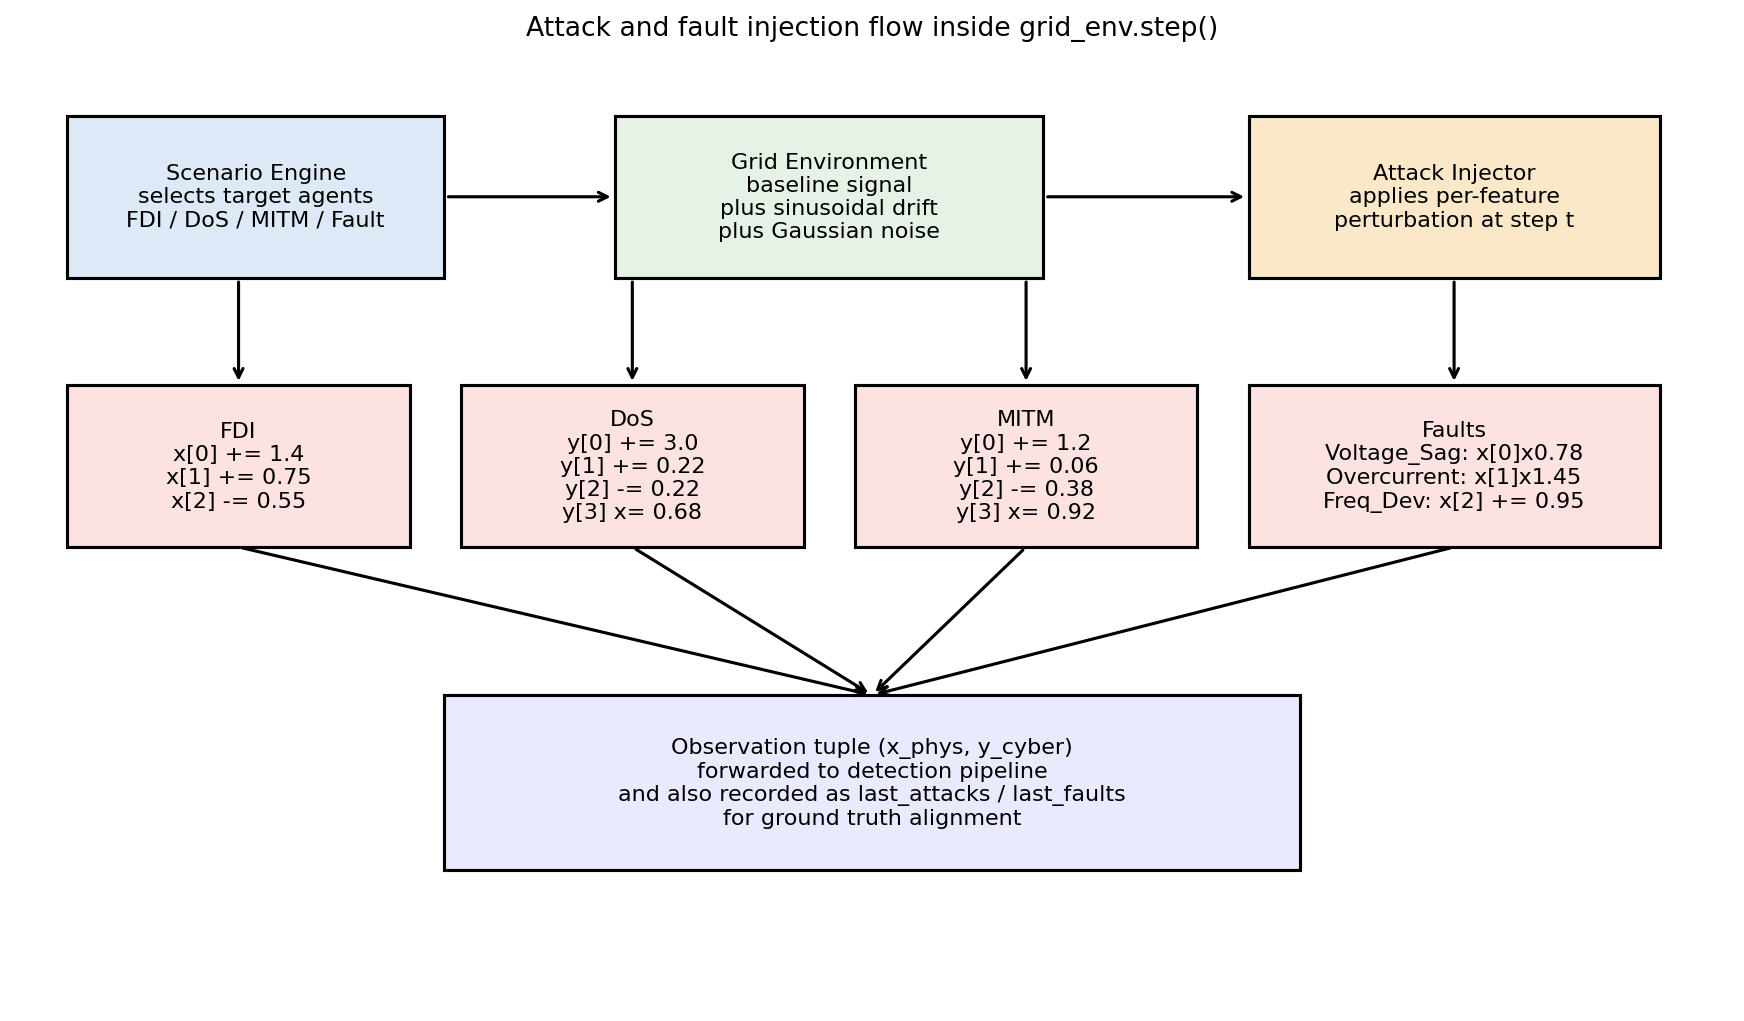
\includegraphics[width=0.95\textwidth]{Fig_AnomalyInjection_Flow.png}}
\caption{Attack and fault injection flow inside the grid environment. The scenario engine selects target agents, the environment produces the baseline signal, and the attack injector applies per feature perturbations before the observation is handed to the detection pipeline.}
\label{fig:anomaly_injection_flow}
\end{figure}

\par \vspace{0.25cm}
\noindent
\textbf{False Data Injection (FDI).} The physical feature vector is shifted so that all three sensor channels deviate at once:
\begin{itemize}
    \item $x[0]$ (voltage) gains $+1.4$ with a small sinusoidal drift $0.08\,\sin(2\pi t / 48)$.
    \item $x[1]$ (current) gains $+0.75$.
    \item $x[2]$ (response) loses $-0.55$.
    \item $y[0]$ (latency) gains $+0.35$ as a residual cyber signature.
\end{itemize}
This multi feature shape is what Layer C-1 (CUSUM with shape gate) targets.

\par \vspace{0.25cm}
\noindent
\textbf{Denial of Service (DoS).} The cyber channel is degraded across all four dimensions simultaneously, with a residual bump on the physical current:
\begin{itemize}
    \item $y[0]$ (latency) gains $+3.0$ with sinusoidal drift $0.4\,\sin(2\pi t / 36)$.
    \item $y[1]$ (packet loss) gains $+0.22$, capped at $1.0$.
    \item $y[2]$ (integrity) loses $-0.22$, floored at $0$.
    \item $y[3]$ (communication frequency) is scaled by $0.68$.
    \item $x[1]$ gains $+0.12$ as a small physical side effect.
\end{itemize}
The 2-of-3 corroboration rule in Layer C-2 fires when at least two of these channels exceed the configured weighted score threshold.

\par \vspace{0.25cm}
\noindent
\textbf{Man-in-the-Middle (MITM).} A MITM event tampers integrity strongly while leaving latency and packet loss only mildly disturbed:
\begin{itemize}
    \item $y[0]$ gains $+1.2$.
    \item $y[1]$ gains $+0.06$.
    \item $y[2]$ loses $-0.38$.
    \item $y[3]$ is scaled by $0.92$.
    \item Physical side effects are limited: $x[0]$ gets a small sinusoidal shift, $x[1]$ gains $+0.10$, $x[2]$ loses $-0.08$.
\end{itemize}
The integrity drop combined with the cyber feature jump z score is what Layer C-3 looks for, with a guard that vetoes the fire when the DoS signature is also present.

\par \vspace{0.25cm}
\noindent
\textbf{Physical Faults.} Three fault types are injected through the same scenario engine. Their signatures dominate one physical feature while leaving the cyber channel almost untouched:
\begin{itemize}
    \item \textit{Voltage Sag.} $x[0]$ is multiplied by $0.78$, $x[1]$ gains $+0.18$, and $y[0]$ gains $+0.30$.
    \item \textit{Overcurrent.} $x[1]$ is multiplied by $1.45$, $x[0]$ gains $+0.12$, and $y[0]$ gains $+0.20$.
    \item \textit{Frequency Deviation.} $x[2]$ gains $+0.95$, $x[1]$ gains $+0.15$, and $y[0]$ gains $+0.15$.
\end{itemize}
These shapes are the basis for the new Layer C-4 fault signature detector described in Chapter~3.

%.....................................................................
\subsection{Anomaly Generation in the Rapid SCADA Live Module}
\label{sec:scada_anomaly}
%.....................................................................

The Rapid SCADA live module does not use \texttt{grid\_env.step()}. Instead, the 100 agent grid is realised as 670 calculated channels distributed across two configuration files, \texttt{Cnl.xml} for the physical channels (300 channels, including one anomaly score channel per agent) and \texttt{Cnl\_Cyber\_Addon.xml} for the cyber channels (370 channels). Every channel carries a Rapid SCADA input formula that produces a continuous, bounded value as a function of the server clock, so the live workspace can be exercised end to end without any physical field device attached.

\par \vspace{0.25cm}
\noindent
The formulas are periodic with a small per agent phase offset so that no two agents move in lockstep. For the first generator the physical and cyber channels use the following formulas (later agents reuse the same shapes with an incremented phase term):
\begin{itemize}
    \item Voltage: $230 + 1.80\,\sin(\text{Now}\cdot 40)$.
    \item Current: $13 + 2.20\,\cos(\text{Now}\cdot 38)$.
    \item Anomaly score: $|\sin(\text{Now}\cdot 12)|\cdot 0.22$.
    \item Latency: $3.0 + |\sin(\text{Now}\cdot 15)|\cdot 0.55$.
    \item Packet loss: $0.001 + |\cos(\text{Now}\cdot 11)|\cdot 0.0025$.
    \item Integrity: $1.0 - |\sin(\text{Now}\cdot 9)|\cdot 0.0150$.
    \item Communication frequency: $50.0 - |\cos(\text{Now}\cdot 13)|\cdot 2.20$.
\end{itemize}

\par \vspace{0.25cm}
\noindent
This calculated channel scheme generates realistic looking telemetry that oscillates within operational bounds and carries a per agent anomaly score, which lets the live dashboard, the PowerShell bridge, the ingestion endpoint, and the detection pipeline be validated against a moving signal. It is important to state plainly that the live module is a telemetry path validator rather than an attack testbed: the discrete FDI, DoS, MITM, and fault events used to measure detection accuracy are injected only in the experiment module described in Section~\ref{sec:attack_injection}. The live module confirms that the data acquisition and visualisation chain works on a continuous SCADA feed, while the experiment module is the source of every quantitative detection result reported in this report. Keeping these two paths separate is what allows the live deployment to be characterised honestly as an operational prototype on calculated channels.

%.....................................................................
\subsection{Evaluation Metrics}
\label{sec:eval_metrics}
%.....................................................................

The following metrics are used to evaluate the performance of the framework across detection accuracy, audit efficiency, and risk management dimensions.

\par \vspace{0.25cm}
\noindent
\textbf{Attack Reduction:}
\begin{equation}
\text{Attack Reduction} = \frac{\text{baseline} - \text{dynamic}}{\text{baseline}}
\label{eq:attack_reduction}
\end{equation}
where $\text{baseline}$ is the number of successful attacks under static auditing and $\text{dynamic}$ is the number under the proposed dynamic scheduling.

\par \vspace{0.25cm}
\noindent
\textbf{Cost Efficiency:}
\begin{equation}
\text{Cost Efficiency} = \frac{\text{baseline\_cost} - \text{dynamic\_cost}}{\text{baseline\_cost}}
\label{eq:cost_efficiency}
\end{equation}

\par \vspace{0.25cm}
\noindent
\textbf{Risk Mitigation:}
\begin{equation}
\text{Risk Mitigation} = \frac{\text{raw\_risk} - \text{effective\_risk}}{\text{raw\_risk}}
\label{eq:risk_mitigation}
\end{equation}

\par \vspace{0.25cm}
\noindent
\textbf{Classification Accuracy:}
\begin{equation}
\text{Accuracy} = \frac{TP + TN}{TP + TN + FP + FN}
\label{eq:accuracy}
\end{equation}
where $TP$, $TN$, $FP$, and $FN$ denote true positives, true negatives, false positives, and false negatives, respectively.

\par \vspace{0.25cm}
\noindent
\textbf{Recall (Sensitivity):}
\begin{equation}
\text{Recall} = \frac{TP}{TP + FN}
\label{eq:recall}
\end{equation}

\par \vspace{0.25cm}
\noindent
\textbf{F1 Score:}
\begin{equation}
\text{F1} = \frac{2 \cdot \text{Precision} \cdot \text{Recall}}{\text{Precision} + \text{Recall}}
\label{eq:f1}
\end{equation}


%---------------------------------------------------------------------
\section{System Integration Workflow}
\label{sec:integration}
%---------------------------------------------------------------------

The end-to-end integration workflow connects all subsystems into a unified operational pipeline. The workflow proceeds through five sequential stages.

\par \vspace{0.35cm}
\noindent
\textbf{Stage 1: Telemetry Generation:} Rapid SCADA generates telemetry data through 670 calculated channels, representing the physical and cyber state of the 100-agent grid. The channels are updated at the configured polling interval, producing a continuous stream of supervisory data within the SCADA environment.

\par \vspace{0.35cm}
\noindent
\textbf{Stage 2: Bridge Retrieval:} The PowerShell bridge script (\mbox{\texttt{pull\_rapidscada\_to\_api.ps1}}) authenticates with the Rapid SCADA Web API at \texttt{127.0.0.1:10109}, retrieves the current channel values in batch, and formats them as a structured JSON payload. The bridge operates on a polling cycle, retrieving updated values at regular intervals.

\par \vspace{0.35cm}
\noindent
\textbf{Stage 3: Batch Transmission:} The formatted telemetry payload is transmitted via HTTP POST to the FastAPI backend ingestion endpoint. The batch transmission approach reduces the number of network round-trips compared to per-agent requests and ensures that all agent data for a given time step arrives atomically.

\par \vspace{0.35cm}
\noindent
\textbf{Stage 4: Backend Processing:} Upon receiving the telemetry batch, the FastAPI backend executes the full detection pipeline in sequence:
\begin{enumerate}
    \item \textit{Feature Mapping}, the raw telemetry values are mapped to the per-agent physical and cyber feature vectors.
    \item \textit{LSTM Inference}, the dual-branch LSTM model produces anomaly probabilities for each agent.
    \item \textit{Deviation Scoring}, physical and cyber deviations are computed against baseline values.
    \item \textit{Multi-Layer Detection}, the three-layer detection architecture (calibrated threshold, temporal accumulator, specialised attack detectors) evaluates each agent.
    \item \textit{Audit Scheduling}, the hybrid scheduler (Q-learning and gradient optimisation) determines updated audit frequencies.
    \item \textit{XAI Generation}, per-agent explainability outputs are computed for both feature domains.
\end{enumerate}

\par \vspace{0.35cm}
\noindent
\textbf{Stage 5: Dashboard Delivery:} The processed results, including anomaly flags, risk scores, audit decisions, escalation actions, and feature-level explanations, are made available to the Next.js dashboard via API responses. The dashboard renders these results in real time, so the operator has a clear view of system health, detection outcomes, and audit decisions.

\begin{figure}[H]
\centering
\fbox{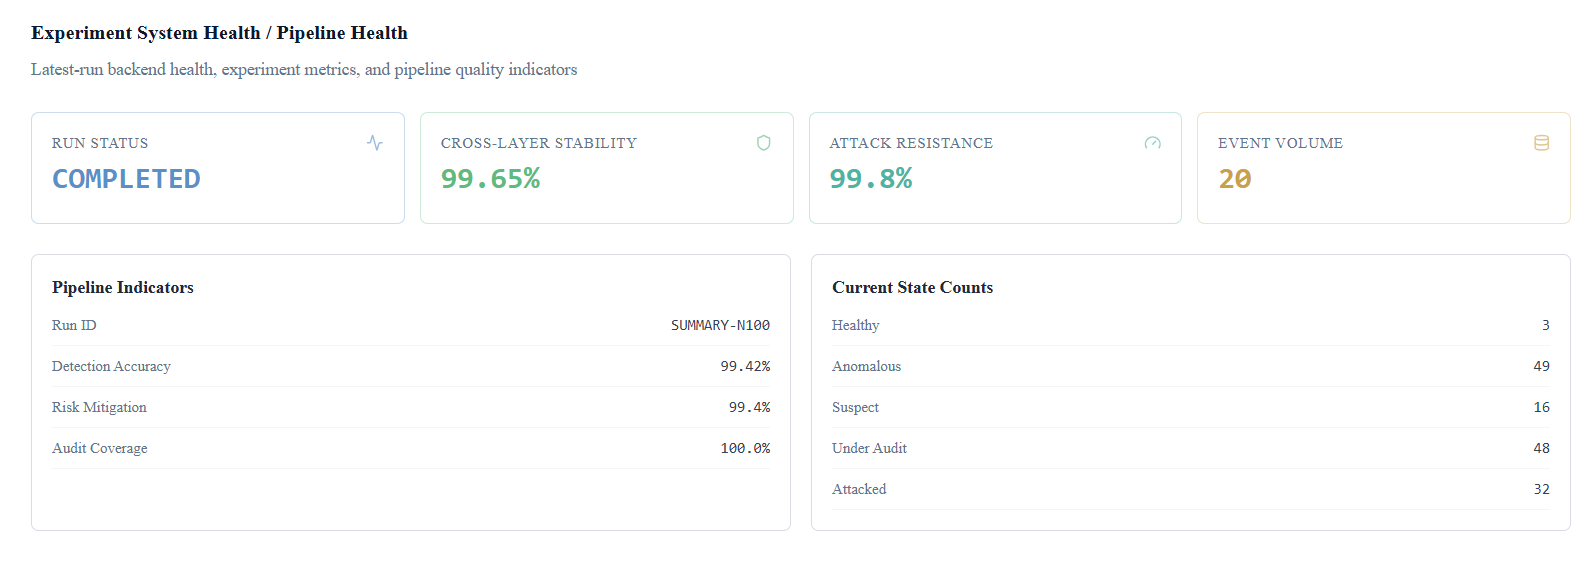
\includegraphics[width=0.95\textwidth]{FigExperiment_System_Health_Pipeline_Health.png}}
\caption{System health and pipeline health view from the dashboard, showing real-time status indicators for each subsystem in the integration workflow.}
\label{fig:system_health}
\end{figure}


%---------------------------------------------------------------------
\section{Feature-wise Functional Mapping}
\label{sec:feature_mapping}
%---------------------------------------------------------------------

Table~\ref{tab:feature_mapping} presents a consolidated mapping of all feature categories used in the framework, together with representative examples and their functional roles within the system.

\begin{table}[H]
\centering
\caption{Feature-wise functional mapping of the SmartGrid AI Audit Framework.}
\label{tab:feature_mapping}
\renewcommand{\arraystretch}{1.3}
\begin{tabularx}{\textwidth}{|l|X|X|}
\hline
\textbf{Feature Category} & \textbf{Example Features} & \textbf{Role in System} \\
\hline
Physical Parameters & Voltage, current, frequency, power, response time & Physical deviation scoring; input to grid branch of LSTM \\
\hline
Cyber Parameters & Latency, packet loss, integrity, communication frequency & Cyber anomaly scoring; input to network branch of LSTM \\
\hline
Baseline Values & Type-specific expected normals for each agent class & Reference for healthy behaviour; denominator in deviation computation \\
\hline
Criticality Weights & GEN, SUB, PMU, BRK class weights & Risk prioritisation; scaling factor in composite score $S_i(t)$ \\
\hline
LSTM Probabilities & anomaly\_prob, grid\_anomaly\_prob, network\_intrusion\_prob & Temporal detection; input to hybrid confidence ensemble \\
\hline
Risk Scores & Deviation-derived and LSTM-derived scores & Audit escalation trigger; input to scheduling and response modules \\
\hline
Explanatory Features & Top contributing deviations per domain & XAI output; operator-facing ranked feature explanations \\
\hline
Pre-Training Data (LSTM) & UCI grid stability (physical branch), UNSW-NB15 (cyber branch) & Initialise LSTM weights before synthetic fine-tuning; no role in live telemetry \\
\hline
\end{tabularx}
\end{table}

\par \vspace{0.35cm}
\noindent
Table~\ref{tab:feature_mapping} shows how information flows through the framework: raw physical and cyber parameters come in from the SCADA layer, get compared against baselines using criticality-weighted deviation scoring, run through the dual-branch LSTM for temporal analysis, combine into risk scores for audit scheduling, and break down into per-feature explanations for operator transparency. Each feature category has a distinct role, so every pipeline stage has traceable inputs and interpretable outputs.
